\documentclass[11pt,a4paper]{report}

\usepackage[utf8]{inputenc}
\usepackage[T1]{fontenc}
\usepackage{textcomp}

\usepackage{parskip}
\usepackage{multicol}
\usepackage{titlesec}
\usepackage{fancyhdr}
\usepackage{fancyvrb}

\usepackage{amsmath}
\usepackage{amssymb}
\usepackage{tocloft}
\usepackage{graphicx}
\usepackage{rotfloat}

\title{Style Based Drawn Artwork Image Classification}
\author{A dissertation submitted in partial fulfilment of the requirements\\
  for the MSc in Intelligent Technologies\\
  \\
  by Michal Grochmal
  $<$\href{mailto:grochmal@member.fsf.org}{grochmal@member.fsf.org}$>$\\
  \\
  Department of Computer Science and Information Systems\\
  Birkbeck College, University of London
}
\date{September 2014}

\usepackage[colorlinks=true]{hyperref}

%\hyphenation{ge-ne-ric Ge-ne-ric Ro-me-ro Ma-ria}

\setlength{\headheight}{16pt}
\renewcommand{\chaptername}{Section}
\renewcommand{\bibname}{References}
\titlespacing*{\chapter}{0pt}{60pt}{60pt}

\titleformat{\chapter}[display]{
  \normalfont\huge\bfseries}{\chaptertitlename\ \thechapter}{20pt}{\Huge}
\titleformat{\section}[block]{
  \normalfont\Large\bfseries}{\thesection}{1em}{}
\titleformat{\subsection}[block]{
  \normalfont\large\bfseries}{\thesubsection}{1em}{}

\begin{document}
\maketitle

\newpage
\null
\thispagestyle{empty}
\newpage

\pagestyle{fancy}
\lhead{}
\chead{STYLE BASED DRAWN ARTWORK IMAGE CLASSIFICATION}
\rhead{}

\begin{abstract}

The abstract of the work, this will be writen at the very end

\begin{flushright}
\emph{Ars longa, vita brevis -- Hippocrates}
\end{flushright}
\end{abstract}

\newpage
\null
\thispagestyle{empty}
\newpage

\newpage
\phantomsection
\addcontentsline{toc}{chapter}{Table of Contents}
\setcounter{page}{1}
\pagenumbering{roman}
\tableofcontents

\newpage
\phantomsection
\addcontentsline{toc}{chapter}{List of Figures}
\listoffigures

\newpage
\phantomsection
\addcontentsline{toc}{chapter}{List of Tables}
\listoftables

\newpage
\phantomsection
\addcontentsline{toc}{chapter}{Academic Declaration}
\chapter*{Academic Declaration}
This report is substantially the result...

\newpage
\phantomsection
\addcontentsline{toc}{chapter}{Acknowledgements}
\chapter*{Acknowledgements}
Thanks to someone here.

\newpage
\setcounter{page}{1}
\pagenumbering{arabic}

\chapter{Introduction}

\begin{multicols}{2}

\section{Background}

Same stuff as in the proposal, just shorter.

Although completely ignoring the content of an image is probably impossible,
features that are independent of the objects in the image exist.  Such features
are more relevant in works of art \cite{zirnhelt07art} as the meaning of how
objects are drawn is important for how humans see a piece of art
\cite{mach10clas}.  In this work, we will use \emph{aesthetic features} tried
on collections of drawn artwork (illustration, drawing and painting) and on
collections of photography, and apply them for classification of artwork with
the meaning of identifying the author of the artwork.  Further, we will try to
extrapolate the meaning of these features and try to identify images of the
same art school and same art period.

nanan nanan nanan nanan nanan nanan nanan nanan nanan nanan nanan nanan nanan
nanan nanan nanan nanan nanan nanan nanan nanan nanan nanan nanan nanan nanan
nanan nanan nanan nanan nanan nanan nanan nanan nanan nanan nanan nanan nanan
nanan nanan nanan nanan nanan nanan nanan nanan nanan nanan nanan nanan nanan
nanan nanan nanan nanan nanan nanan nanan nanan nanan nanan nanan nanan nanan
nanan nanan nanan nanan nanan nanan nanan nanan nanan nanan nanan nanan nanan
nanan nanan nanan nanan nanan nanan nanan nanan nanan nanan nanan nanan nanan
nanan nanan nanan nanan nanan nanan nanan nanan nanan nanan nanan nanan nanan
nanan nanan nanan nanan nanan nanan nanan nanan nanan nanan nanan nanan nanan
batman

\begin{figure*}[tb]  % figre* instead of figure becuse of multicols
\centering
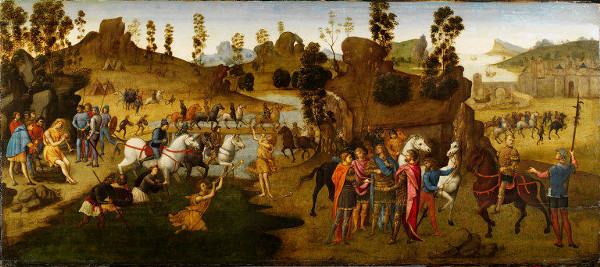
\includegraphics[width=0.48\textwidth]{diff_caesar}
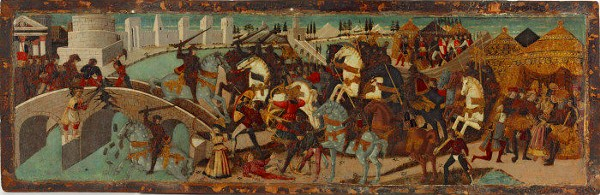
\includegraphics[width=0.48\textwidth]{diff_horatius}
\caption[Example of different styles]{The image at the top is the painting
"Julius Caesar and the Crossing of the Rubicon" by Francesco Granacci and at
the bottom is the panel "Horatius Cocles Defending the Sublician Bridge" by
Francesco Pesellino.  Both images have a similar theme and the objects
contained in them are similar, yet the style of the images is different.}
\label{diff}
\end{figure*}

\begin{figure*}[tb]
\centering
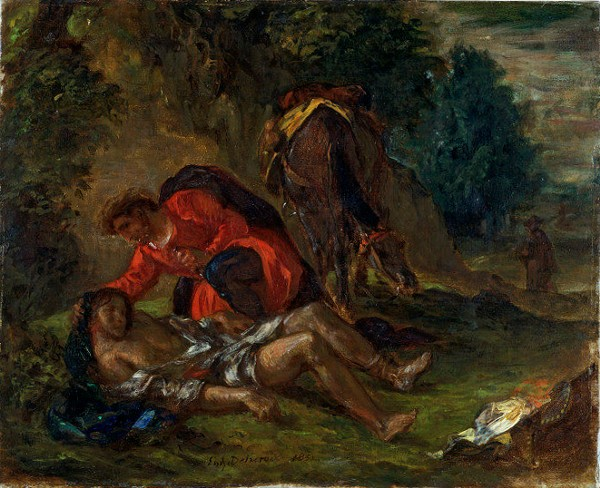
\includegraphics[width=0.48\textwidth]{sim_delacroix_samaritan}
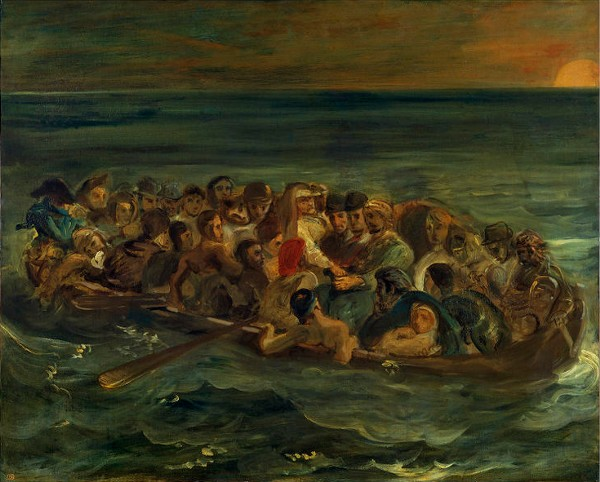
\includegraphics[width=0.48\textwidth]{sim_delacroix_shipwreck}
\caption[Example of similar styles]{In these two paintings by Delacroix, "The
Good Samaritan" and "The Shipwreck of Don Juan", we can see a similar style.
Both paintings are different in their theme, yet the author's style of drawing
and painting can be easily noticed by humans.}
\label{similar}
\end{figure*}

\section{Features in the previous works}

Description of features in Romeo's work \cite{rmc12ajs} and in Machajdik's work
\cite{mach10clas}.  Describing ignored features too (and why they were
ignored).

nanan nanan nanan nanan nanan nanan nanan nanan nanan nanan nanan nanan nanan
nanan nanan nanan nanan nanan nanan nanan nanan nanan nanan nanan nanan nanan
nanan nanan nanan nanan nanan nanan nanan nanan nanan nanan nanan nanan nanan
nanan nanan nanan nanan nanan nanan nanan nanan nanan nanan nanan nanan nanan
nanan nanan nanan nanan nanan nanan nanan nanan nanan nanan nanan nanan nanan
nanan nanan nanan nanan nanan nanan nanan nanan nanan nanan nanan nanan nanan
nanan nanan nanan nanan nanan nanan nanan nanan nanan nanan nanan nanan nanan
nanan nanan nanan nanan nanan nanan nanan nanan nanan nanan nanan nanan nanan
nanan nanan nanan nanan nanan nanan nanan nanan nanan nanan nanan nanan nanan
batman

\end{multicols}

\chapter{Acquiring datasets}

\begin{multicols}{2}

\section{Victoria and Albert Museum (VAM)}

VAM exposes a JSON API to retrieve metadata and image locations, the metadata
is organised as a small JSON structure for each museum item.

`vam-get-all.py` used to get metadata about all items in the category
painintins.  Yielding 2000 results.

Using `jgrep` the results were filtered into 878 items with an availlable
image.

Downloaded the images using `vam-img-get.py` and filtered the images by hand
removing 10 images that were not of painintgs.  Giving a final result of 868
images of paintings with metadata.

\section{Visual Arts Data Service (NIRP)}

Visual Arts Data Service, Nice Paintings - VADS NIRP

Searched the alphabetical index of artists using `all-artists.py`, giving us
3222 artists.

Each artist was checked for works and artists without works (23 such artists
were present) were filtered out.  This was achieved with `curl` and `grep`.

The artist index on NIRP contains duplicate entries for the same artist and
names that are categories of artists (e.g. "French painters").  This result in
individual painitngs being listed several times, we deal with it later.

`by-artist.py` was used to retrieve detailed pages about all paintings of all
artists.  The duplicates were removed by simple `sort | uniq`.  Yielding 9181
unique paintings.

Finally `get-painting.py` crawls the detail page, retrieves the image for the
painting and converts the HTML representation of the metadata into a JSON
representation.

In a JSON representation the painings that do not have an image available were
filtered out using `jgrep`.

\section{Further cleansing}

Semi automatic check for duplicated by checking if no two images have the same
sha1sum checksum.  Use of jgrep, jcut, etc to perfom artist cleaing...

nanan nanan nanan nanan nanan nanan nanan nanan nanan nanan nanan nanan nanan
nanan nanan nanan nanan nanan nanan nanan nanan nanan nanan nanan nanan nanan
nanan nanan nanan nanan nanan nanan nanan nanan nanan nanan nanan nanan nanan
nanan nanan nanan nanan nanan nanan nanan nanan nanan nanan nanan nanan nanan
nanan nanan nanan nanan nanan nanan nanan nanan nanan nanan nanan nanan nanan
nanan nanan nanan nanan nanan nanan nanan nanan nanan nanan nanan nanan nanan
nanan nanan nanan nanan nanan nanan nanan nanan nanan nanan nanan nanan nanan
nanan nanan nanan nanan nanan nanan nanan nanan nanan nanan nanan nanan nanan
nanan nanan nanan nanan nanan nanan nanan nanan nanan nanan nanan nanan nanan
batman

\end{multicols}

\chapter{Methodology}

\begin{multicols}{2}

\section{Normalisation and separation}

First of all size normalisation, as most features depend on the number of
pixels in the image.  As close as possible to 300 000 pixels but without
changing the aspect ration.  In golden ration 300 000 pixels is an image of
671x447 pixels, it is close to the ASCII screen resolution of 640x480 pixels.
Equation \ref{eqsize} shows how an image of arbitrary \emph{height} and
\emph{width} can be resized to an image of 300 000 pixels.  This technique do
not ensures that an image will have the desired number of pixels but that it
will be as close as possible to 300 000 pixels without changing the spect
ration.  In our dataset the image that deviated the most ended with 299 485
pixels, that's an error of less than 0.172\% and, therefore, can be ignored.

\begin{equation}
\begin{aligned}
height'  &= height \times \sqrt{ \frac{3 \times 10^5}{height \times width} } \\
width'   &= width  \times \sqrt{ \frac{3 \times 10^5}{height \times width} } \\
\label{eqsize}
\end{aligned}
\end{equation}

\begin{figure*}[tbp]
\centering
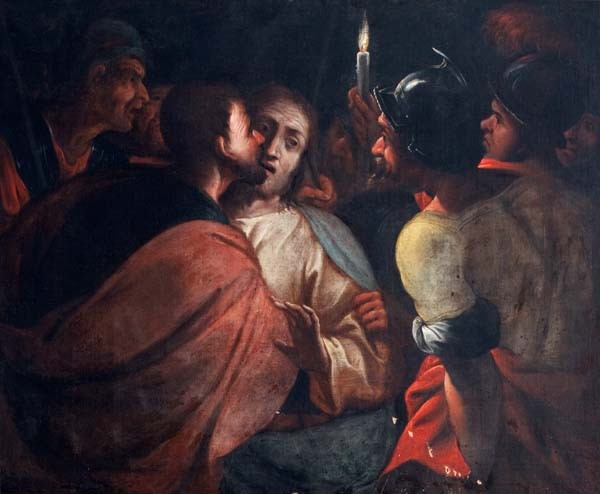
\includegraphics[width=0.48\textwidth]{nirp_caravaggio_1962_139_1}
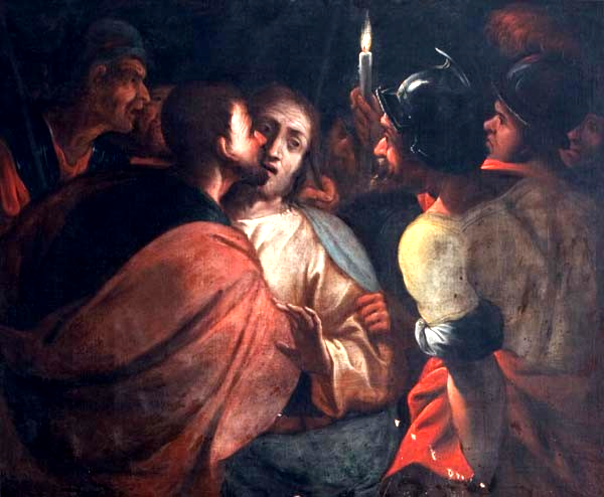
\includegraphics[width=0.48\textwidth]{caravaggio_1962_139_1}
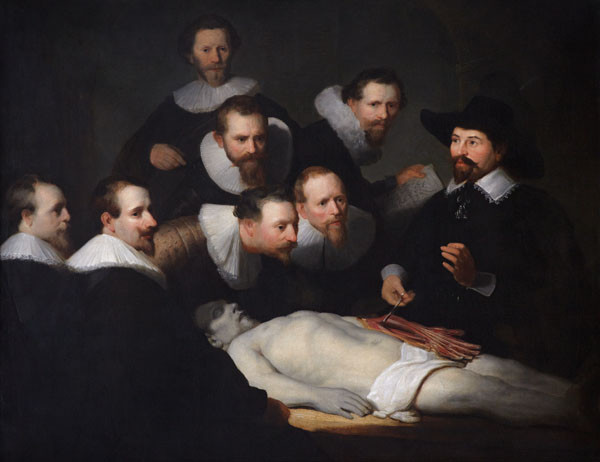
\includegraphics[width=0.48\textwidth]{nirp_rembrandt_eu_464}
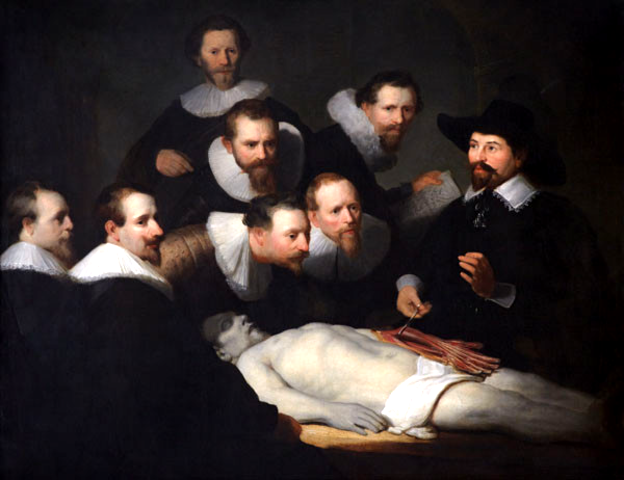
\includegraphics[width=0.48\textwidth]{rembrandt_eu_464}
\caption[Colour normalisation]{To the left original image, to the right
normalised one.}
\label{norm}
\end{figure*}

Different pictures of the same painting may have different illumination, colour
normalisation removes this complexity.  Colour normalisation is performed by,
for each channel, subtracting the minimum value from all pixels, then dividing
them by the value of the maximum value and multiplying by 255.

\begin{figure*}[!htb]
\begin{equation}
\begin{aligned}
H_{HSV}  &= atan2\left(\frac{\sqrt{3}}{2}(G-B), \frac{1}{2}(2R-G-B)\right) \\
V_{HSV}  &= max(R,G,B) \\
S_{HSV}  &= \left\{
  \begin{array}{ll}
    0  &  \text{if } V = 0, \\
    \frac{\sqrt{ \left(\frac{\sqrt{3}}{2}(G-B)\right)^2
               + \left(\frac{1}{2}(2R-G-B)\right)^2 }}{V}
  &  \text{otherwise}. \\
  \end{array}
            \right.
\label{eqhsv}
\end{aligned}
\end{equation}
\end{figure*}

\begin{figure*}[!htb]
\begin{equation}
\begin{aligned}
H_{HSL}  &= atan2\left(\frac{\sqrt{3}}{2}(G-B), \frac{1}{2}(2R-G-B)\right) \\
L_{HSL}  &= \frac{1}{2}max(R,G,B) + \frac{1}{2}min(R,G,B) \\
S_{HSL}  &= \left\{
  \begin{array}{ll}
    0  &  \text{if } L \in \{0,1\}, \\
    \frac{\sqrt{ \left(\frac{\sqrt{3}}{2}(G-B)\right)^2
               + \left(\frac{1}{2}(2R-G-B)\right)^2 }}{1 - \lvert 2L-1 \rvert}
  &  \text{otherwise}. \\
  \end{array}
           \right.
\label{eqhsl}
\end{aligned}
\end{equation}
\end{figure*}

\begin{equation}
CS_{HSV} = \frac{S_{HSV} \times V_{HSV}}{255}
\label{eqcs}
\end{equation}

Usubg equations for HSV \ref{eqhsv}, HSL \ref{eqhsl} and CS \ref{eqcs}.

nanan nanan nanan nanan nanan nanan nanan nanan nanan nanan nanan nanan nanan
nanan nanan nanan nanan nanan nanan nanan nanan nanan nanan nanan nanan nanan
nanan nanan nanan nanan nanan nanan nanan nanan nanan nanan nanan nanan nanan
nanan nanan nanan nanan nanan nanan nanan nanan nanan nanan nanan nanan nanan
nanan nanan nanan nanan nanan nanan nanan nanan nanan nanan nanan nanan nanan
nanan nanan nanan nanan nanan nanan nanan nanan nanan nanan nanan nanan nanan
nanan nanan nanan nanan nanan nanan nanan nanan nanan nanan nanan nanan nanan
nanan nanan nanan nanan nanan nanan nanan nanan nanan nanan nanan nanan nanan
nanan nanan nanan nanan nanan nanan nanan nanan nanan nanan nanan nanan nanan
batman

Separation into HSV and HSL, equations below.  Also, defintion of Romeo's
colourfullness.

\begin{figure*}[tbp]
\centering
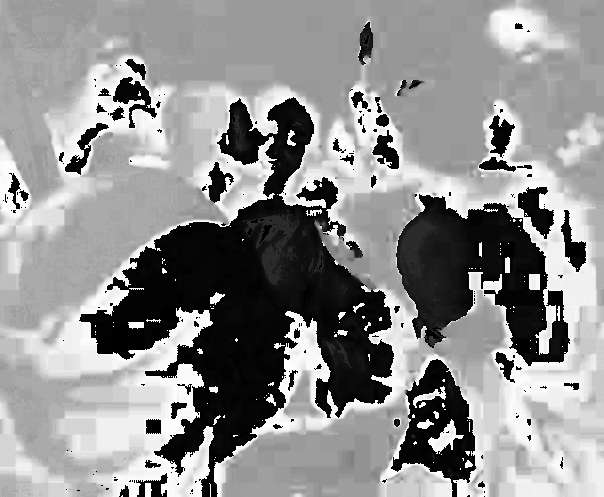
\includegraphics[width=0.30\textwidth]{H_caravaggio_1962_139_1}
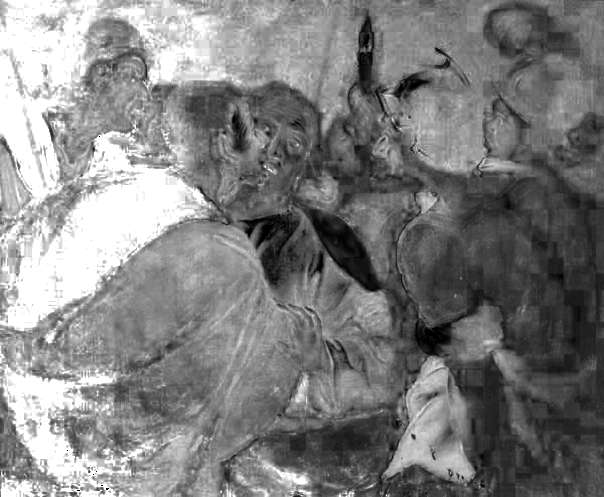
\includegraphics[width=0.30\textwidth]{SHSV_caravaggio_1962_139_1}
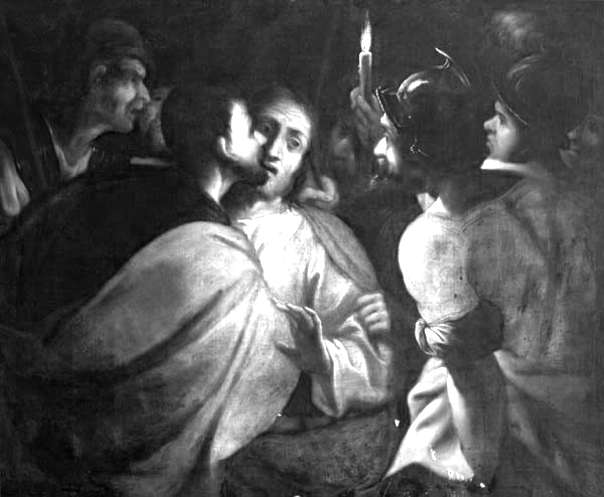
\includegraphics[width=0.30\textwidth]{V_caravaggio_1962_139_1}
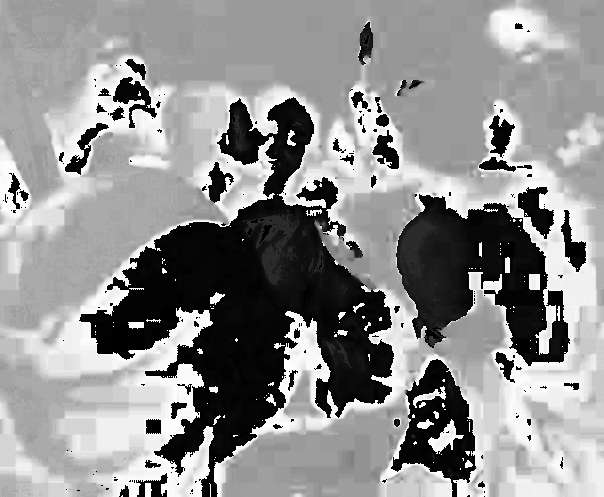
\includegraphics[width=0.30\textwidth]{H_caravaggio_1962_139_1}
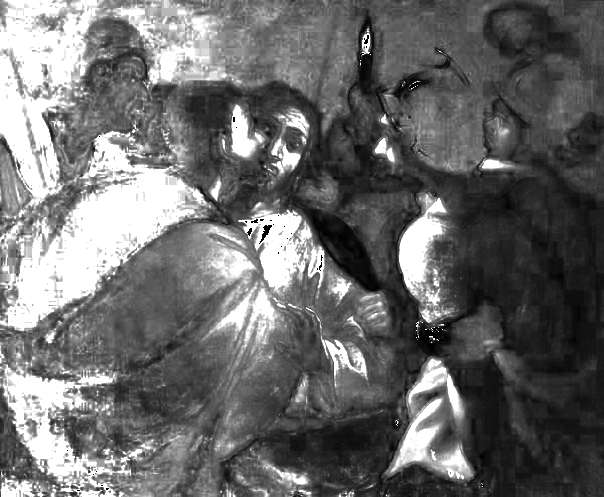
\includegraphics[width=0.30\textwidth]{SHSL_caravaggio_1962_139_1}
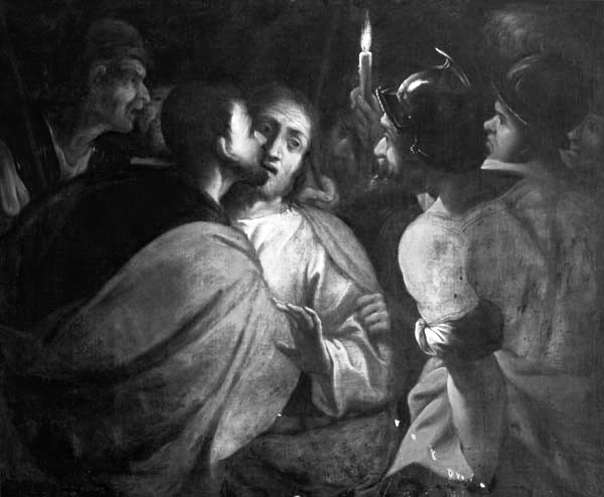
\includegraphics[width=0.30\textwidth]{L_caravaggio_1962_139_1}
\caption[HSV/HSL separation]{HSV/HSL separation}
\label{hsvl}
\end{figure*}

\begin{figure*}[tbp]
\centering
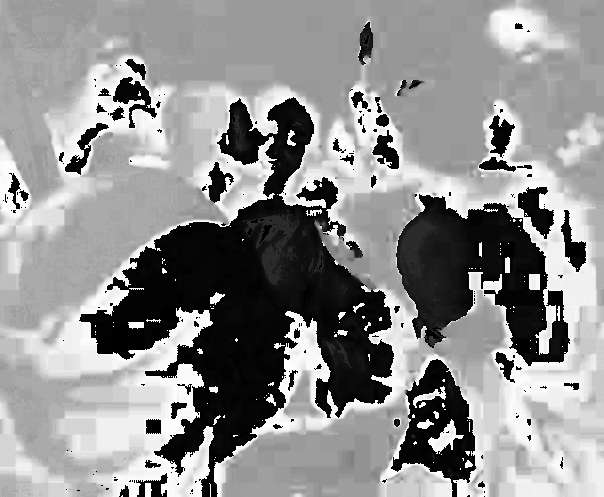
\includegraphics[width=0.30\textwidth]{H_caravaggio_1962_139_1}
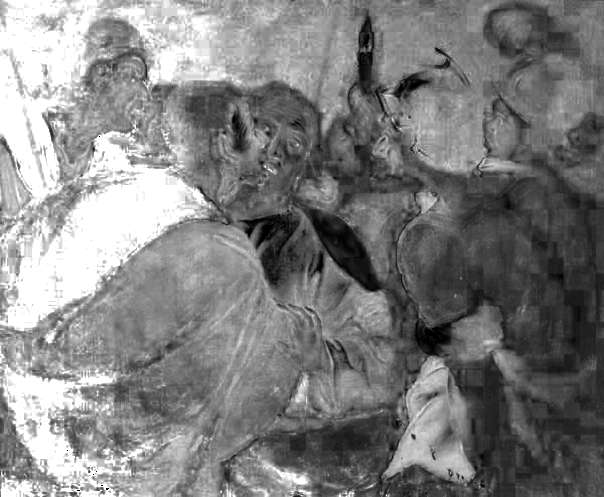
\includegraphics[width=0.30\textwidth]{SHSV_caravaggio_1962_139_1}
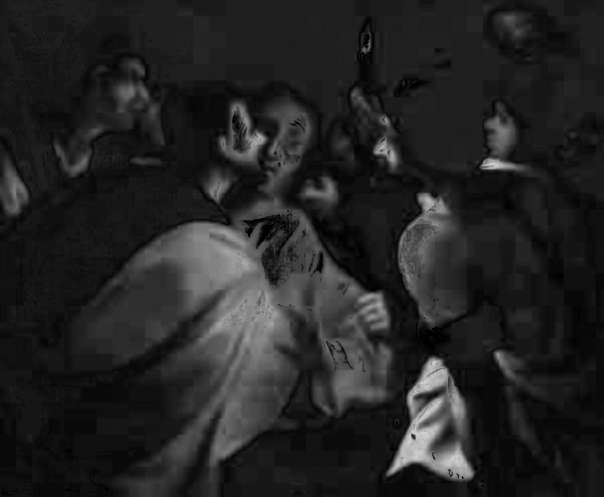
\includegraphics[width=0.30\textwidth]{CS_caravaggio_1962_139_1}
\caption[Colourfullness]{Colourfullness}
\label{figcs}
\end{figure*}

\section{Basic Features}

Groups of related features decribed below.

\subsection{Kolmogorov complexity}

Sobel and Canny filters, JPEG compression

nanan nanan nanan nanan nanan nanan nanan nanan nanan nanan nanan nanan nanan
nanan nanan nanan nanan nanan nanan nanan nanan nanan nanan nanan nanan nanan
nanan nanan nanan nanan nanan nanan nanan nanan nanan nanan nanan nanan nanan
nanan nanan nanan nanan nanan nanan nanan nanan nanan nanan nanan nanan nanan
nanan nanan nanan nanan nanan nanan nanan nanan nanan nanan nanan nanan nanan
nanan nanan nanan nanan nanan nanan nanan nanan nanan nanan nanan nanan nanan
nanan nanan nanan nanan nanan nanan nanan nanan nanan nanan nanan nanan nanan
nanan nanan nanan nanan nanan nanan nanan nanan nanan nanan nanan nanan nanan
nanan nanan nanan nanan nanan nanan nanan nanan nanan nanan nanan nanan nanan
batman

\subsection{Grey Level Co-occurrence Matrix}

All features of texture coming from that.

nanan nanan nanan nanan nanan nanan nanan nanan nanan nanan nanan nanan nanan
nanan nanan nanan nanan nanan nanan nanan nanan nanan nanan nanan nanan nanan
nanan nanan nanan nanan nanan nanan nanan nanan nanan nanan nanan nanan nanan
nanan nanan nanan nanan nanan nanan nanan nanan nanan nanan nanan nanan nanan
nanan nanan nanan nanan nanan nanan nanan nanan nanan nanan nanan nanan nanan
nanan nanan nanan nanan nanan nanan nanan nanan nanan nanan nanan nanan nanan
nanan nanan nanan nanan nanan nanan nanan nanan nanan nanan nanan nanan nanan
nanan nanan nanan nanan nanan nanan nanan nanan nanan nanan nanan nanan nanan
nanan nanan nanan nanan nanan nanan nanan nanan nanan nanan nanan nanan nanan
batman

\begin{figure*}[tbp]
\centering
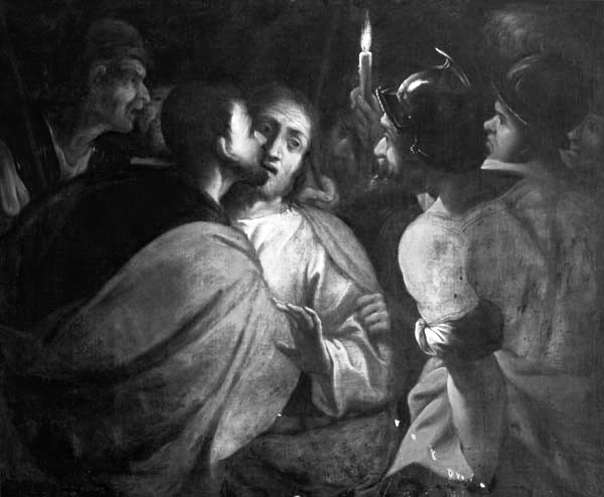
\includegraphics[width=0.30\textwidth]{L_caravaggio_1962_139_1}
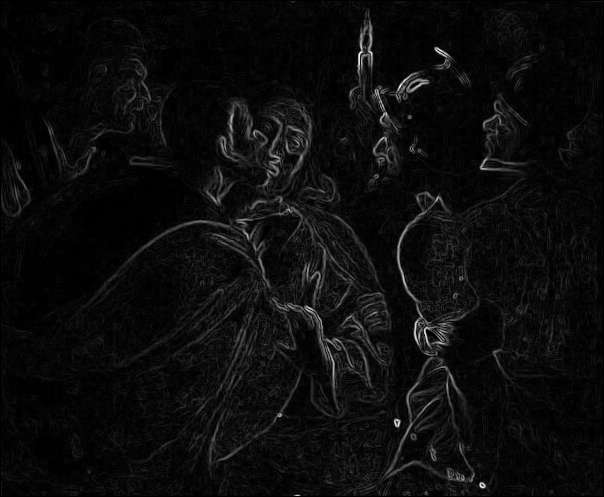
\includegraphics[width=0.30\textwidth]{sobel_L_caravaggio_1962_139_1}
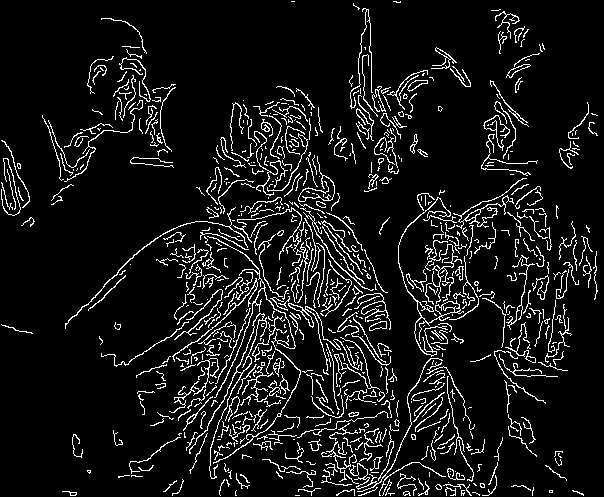
\includegraphics[width=0.30\textwidth]{canny_L_caravaggio_1962_139_1}
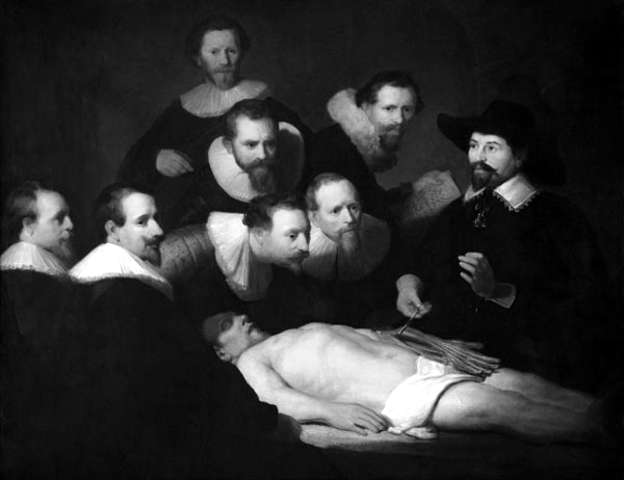
\includegraphics[width=0.30\textwidth]{L_rembrandt_eu_464}
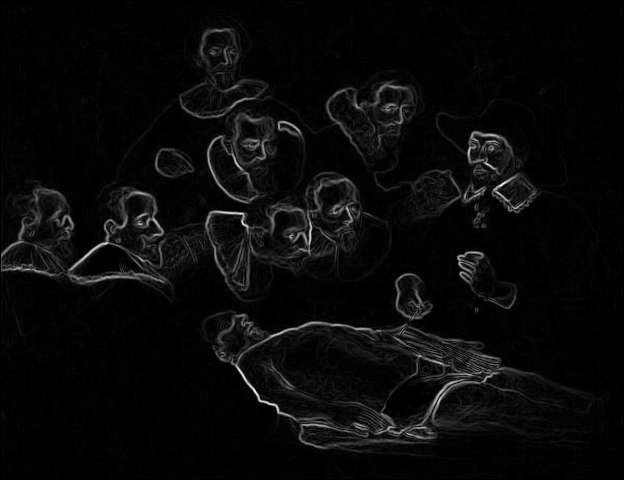
\includegraphics[width=0.30\textwidth]{sobel_L_rembrandt_eu_464}
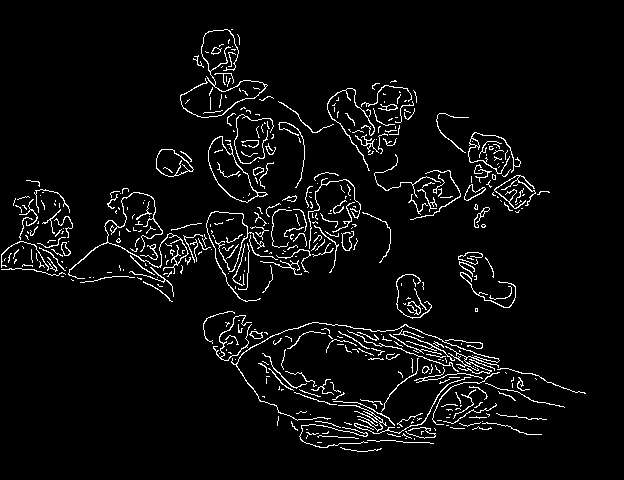
\includegraphics[width=0.30\textwidth]{canny_L_rembrandt_eu_464}
\caption[Canny and Sobel filters of Ligthness]{Canny and Sobel filters of
Lightness}
\label{figcansobl}
\end{figure*}

\begin{figure*}[tbp]
\centering
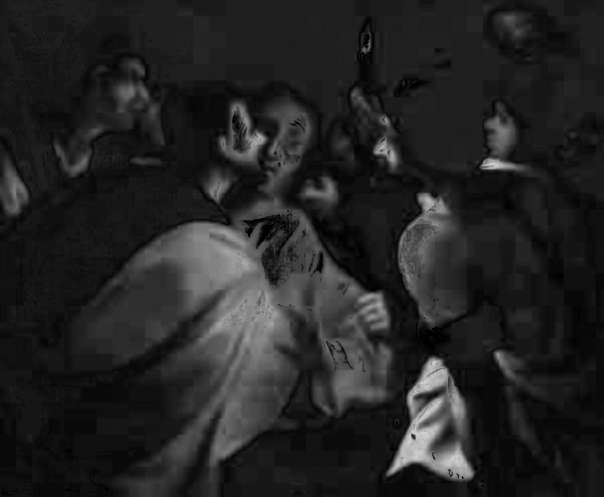
\includegraphics[width=0.30\textwidth]{CS_caravaggio_1962_139_1}
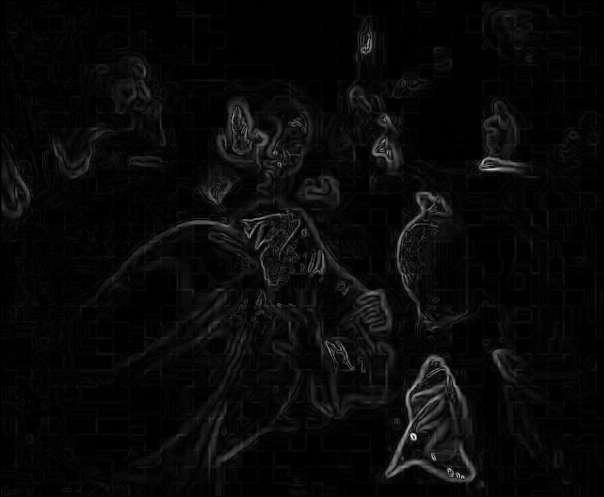
\includegraphics[width=0.30\textwidth]{sobel_CS_caravaggio_1962_139_1}
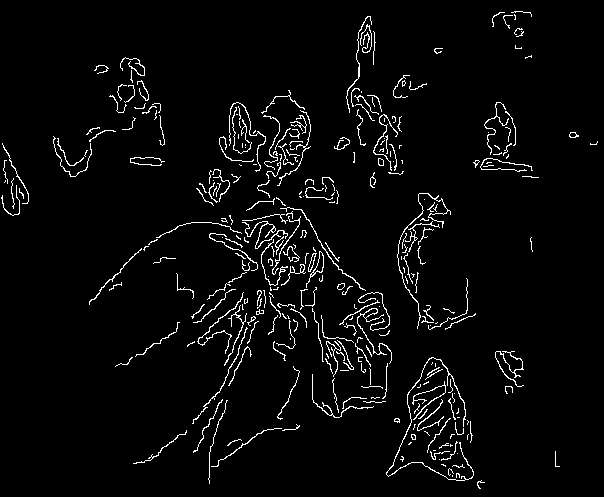
\includegraphics[width=0.30\textwidth]{canny_CS_caravaggio_1962_139_1}
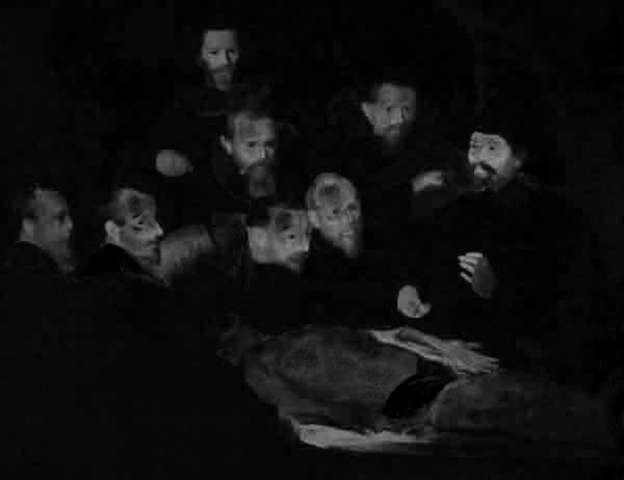
\includegraphics[width=0.30\textwidth]{CS_rembrandt_eu_464}
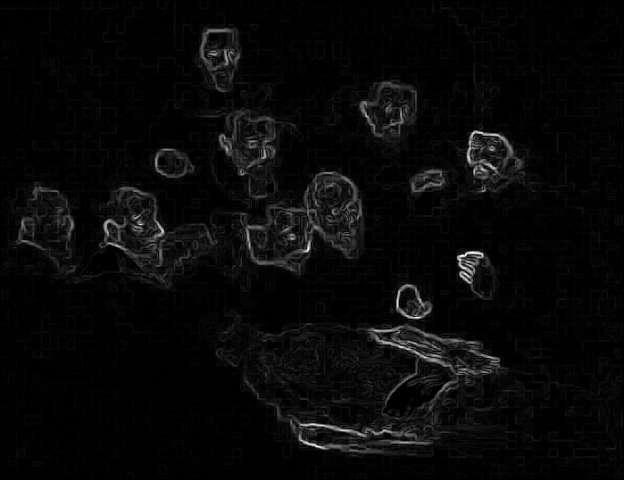
\includegraphics[width=0.30\textwidth]{sobel_CS_rembrandt_eu_464}
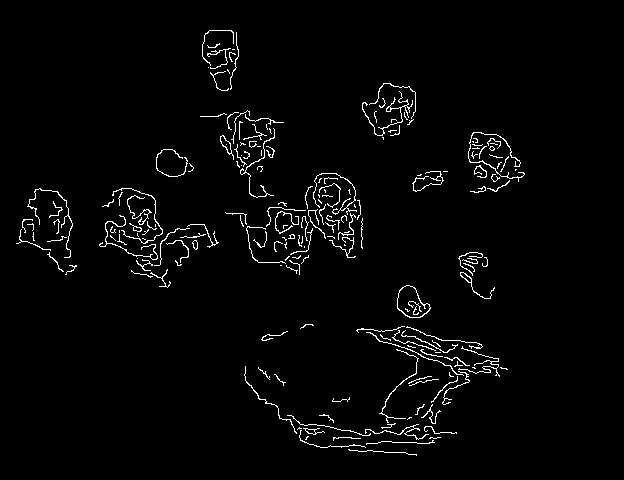
\includegraphics[width=0.30\textwidth]{canny_CS_rembrandt_eu_464}
\caption[Canny and Sobel filters of Colourfullness]{Canny and Sobel filters of
Colourfullness}
\label{figcansobcs}
\end{figure*}

\subsection{Image Averages}

Std and average, super simple.

nanan nanan nanan nanan nanan nanan nanan nanan nanan nanan nanan nanan nanan
nanan nanan nanan nanan nanan nanan nanan nanan nanan nanan nanan nanan nanan
nanan nanan nanan nanan nanan nanan nanan nanan nanan nanan nanan nanan nanan
nanan nanan nanan nanan nanan nanan nanan nanan nanan nanan nanan nanan nanan
nanan nanan nanan nanan nanan nanan nanan nanan nanan nanan nanan nanan nanan
batman

\subsection{Rule of Thirds}

Same averages on the central rectangle.

nanan nanan nanan nanan nanan nanan nanan nanan nanan nanan nanan nanan nanan
nanan nanan nanan nanan nanan nanan nanan nanan nanan nanan nanan nanan nanan
nanan nanan nanan nanan nanan nanan nanan nanan nanan nanan nanan nanan nanan
nanan nanan nanan nanan nanan nanan nanan nanan nanan nanan nanan nanan nanan
nanan nanan nanan nanan nanan nanan nanan nanan nanan nanan nanan nanan nanan
batman

\section{Itten Colours}

Stuff based on itten colours

\subsection{Amount of each colour}

Only the colours above the image average get counted.

nanan nanan nanan nanan nanan nanan nanan nanan nanan nanan nanan nanan nanan
nanan nanan nanan nanan nanan nanan nanan nanan nanan nanan nanan nanan nanan
nanan nanan nanan nanan nanan nanan nanan nanan nanan nanan nanan nanan nanan
nanan nanan nanan nanan nanan nanan nanan nanan nanan nanan nanan nanan nanan
nanan nanan nanan nanan nanan nanan nanan nanan nanan nanan nanan nanan nanan
batman

\subsection{Segmentation}

To measure contrasts we need to segment the image.  Rule of thirds, rule of
seven, watershed segmentation.

nanan nanan nanan nanan nanan nanan nanan nanan nanan nanan nanan nanan nanan
nanan nanan nanan nanan nanan nanan nanan nanan nanan nanan nanan nanan nanan
nanan nanan nanan nanan nanan nanan nanan nanan nanan nanan nanan nanan nanan
nanan nanan nanan nanan nanan nanan nanan nanan nanan nanan nanan nanan nanan
nanan nanan nanan nanan nanan nanan nanan nanan nanan nanan nanan nanan nanan
batman

\subsection{Itten Contrasts}

Contrast of hue, saturation, light and dark, warm and cold colours,
complements.

\begin{figure*}[!htb]
\begin{equation}
\begin{aligned}
n_1       &= max(0.1, 1 - warm_1 - cold_1) \\
n_2       &= max(0.1, 1 - warm_2 - cold_2) \\
contrast  &= \frac{ max\left( \left\lvert \frac{warm_1}{warm_2}
                                        - \frac{cold_1}{cold_2} \right\rvert
                            , \left\lvert \frac{warm_2}{warm_1}
                                        - \frac{cold_2}{cold_1} \right\rvert
                       \right)
                 }{ n_1 \times n_2 }
\label{eqcoldwarm}
\end{aligned}
\end{equation}
\end{figure*}

\begin{figure*}[!htb]
\begin{equation}
\begin{aligned}
n_1       &= 1 - warm_1 - cold_1 \\
n_2       &= 1 - warm_2 - cold_2 \\
contrast  &= \frac{ warm_1 \times warm_2
                   + n_1    \times n_2
                   + cold_1 \times cold_2
                  }{ \sqrt{ (warm_1 + n_1 + cold_1)^2
                          + (warm_2 + n_2 + cold_2)^2 } }
\label{eqmach}
\end{aligned}
\end{equation}
\end{figure*}

\begin{figure*}[!htb]
\begin{equation}
D = min( \lvert H_1 - H_2 \rvert , 360 - \lvert H_1 - H_2 \rvert )
\label{eqwheel}
\end{equation}
\end{figure*}

nanan nanan nanan nanan nanan nanan nanan nanan nanan nanan nanan nanan nanan
nanan nanan nanan nanan nanan nanan nanan nanan nanan nanan nanan nanan nanan
nanan nanan nanan nanan nanan nanan nanan nanan nanan nanan nanan nanan nanan
nanan nanan nanan nanan nanan nanan nanan nanan nanan nanan nanan nanan nanan
nanan nanan nanan nanan nanan nanan nanan nanan nanan nanan nanan nanan nanan
batman

\begin{figure*}[tbp]
\centering
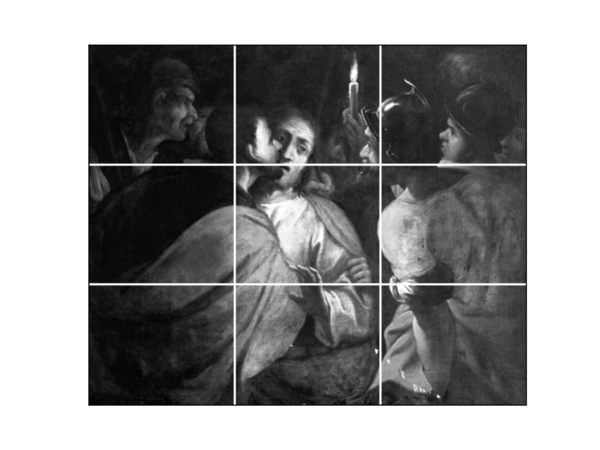
\includegraphics[width=0.48\textwidth]{r3_L_caravaggio_1962_139_1}
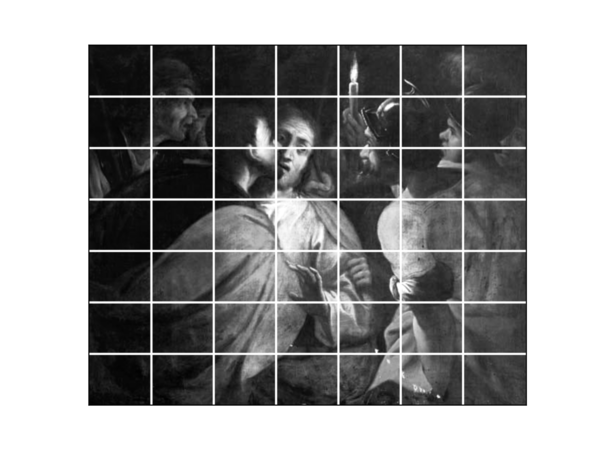
\includegraphics[width=0.48\textwidth]{r7_L_caravaggio_1962_139_1}
\caption[Rule of thirds]{Rule of thirds}
\label{figr3}
\end{figure*}

\begin{sidewaysfigure*}[p]
\centering
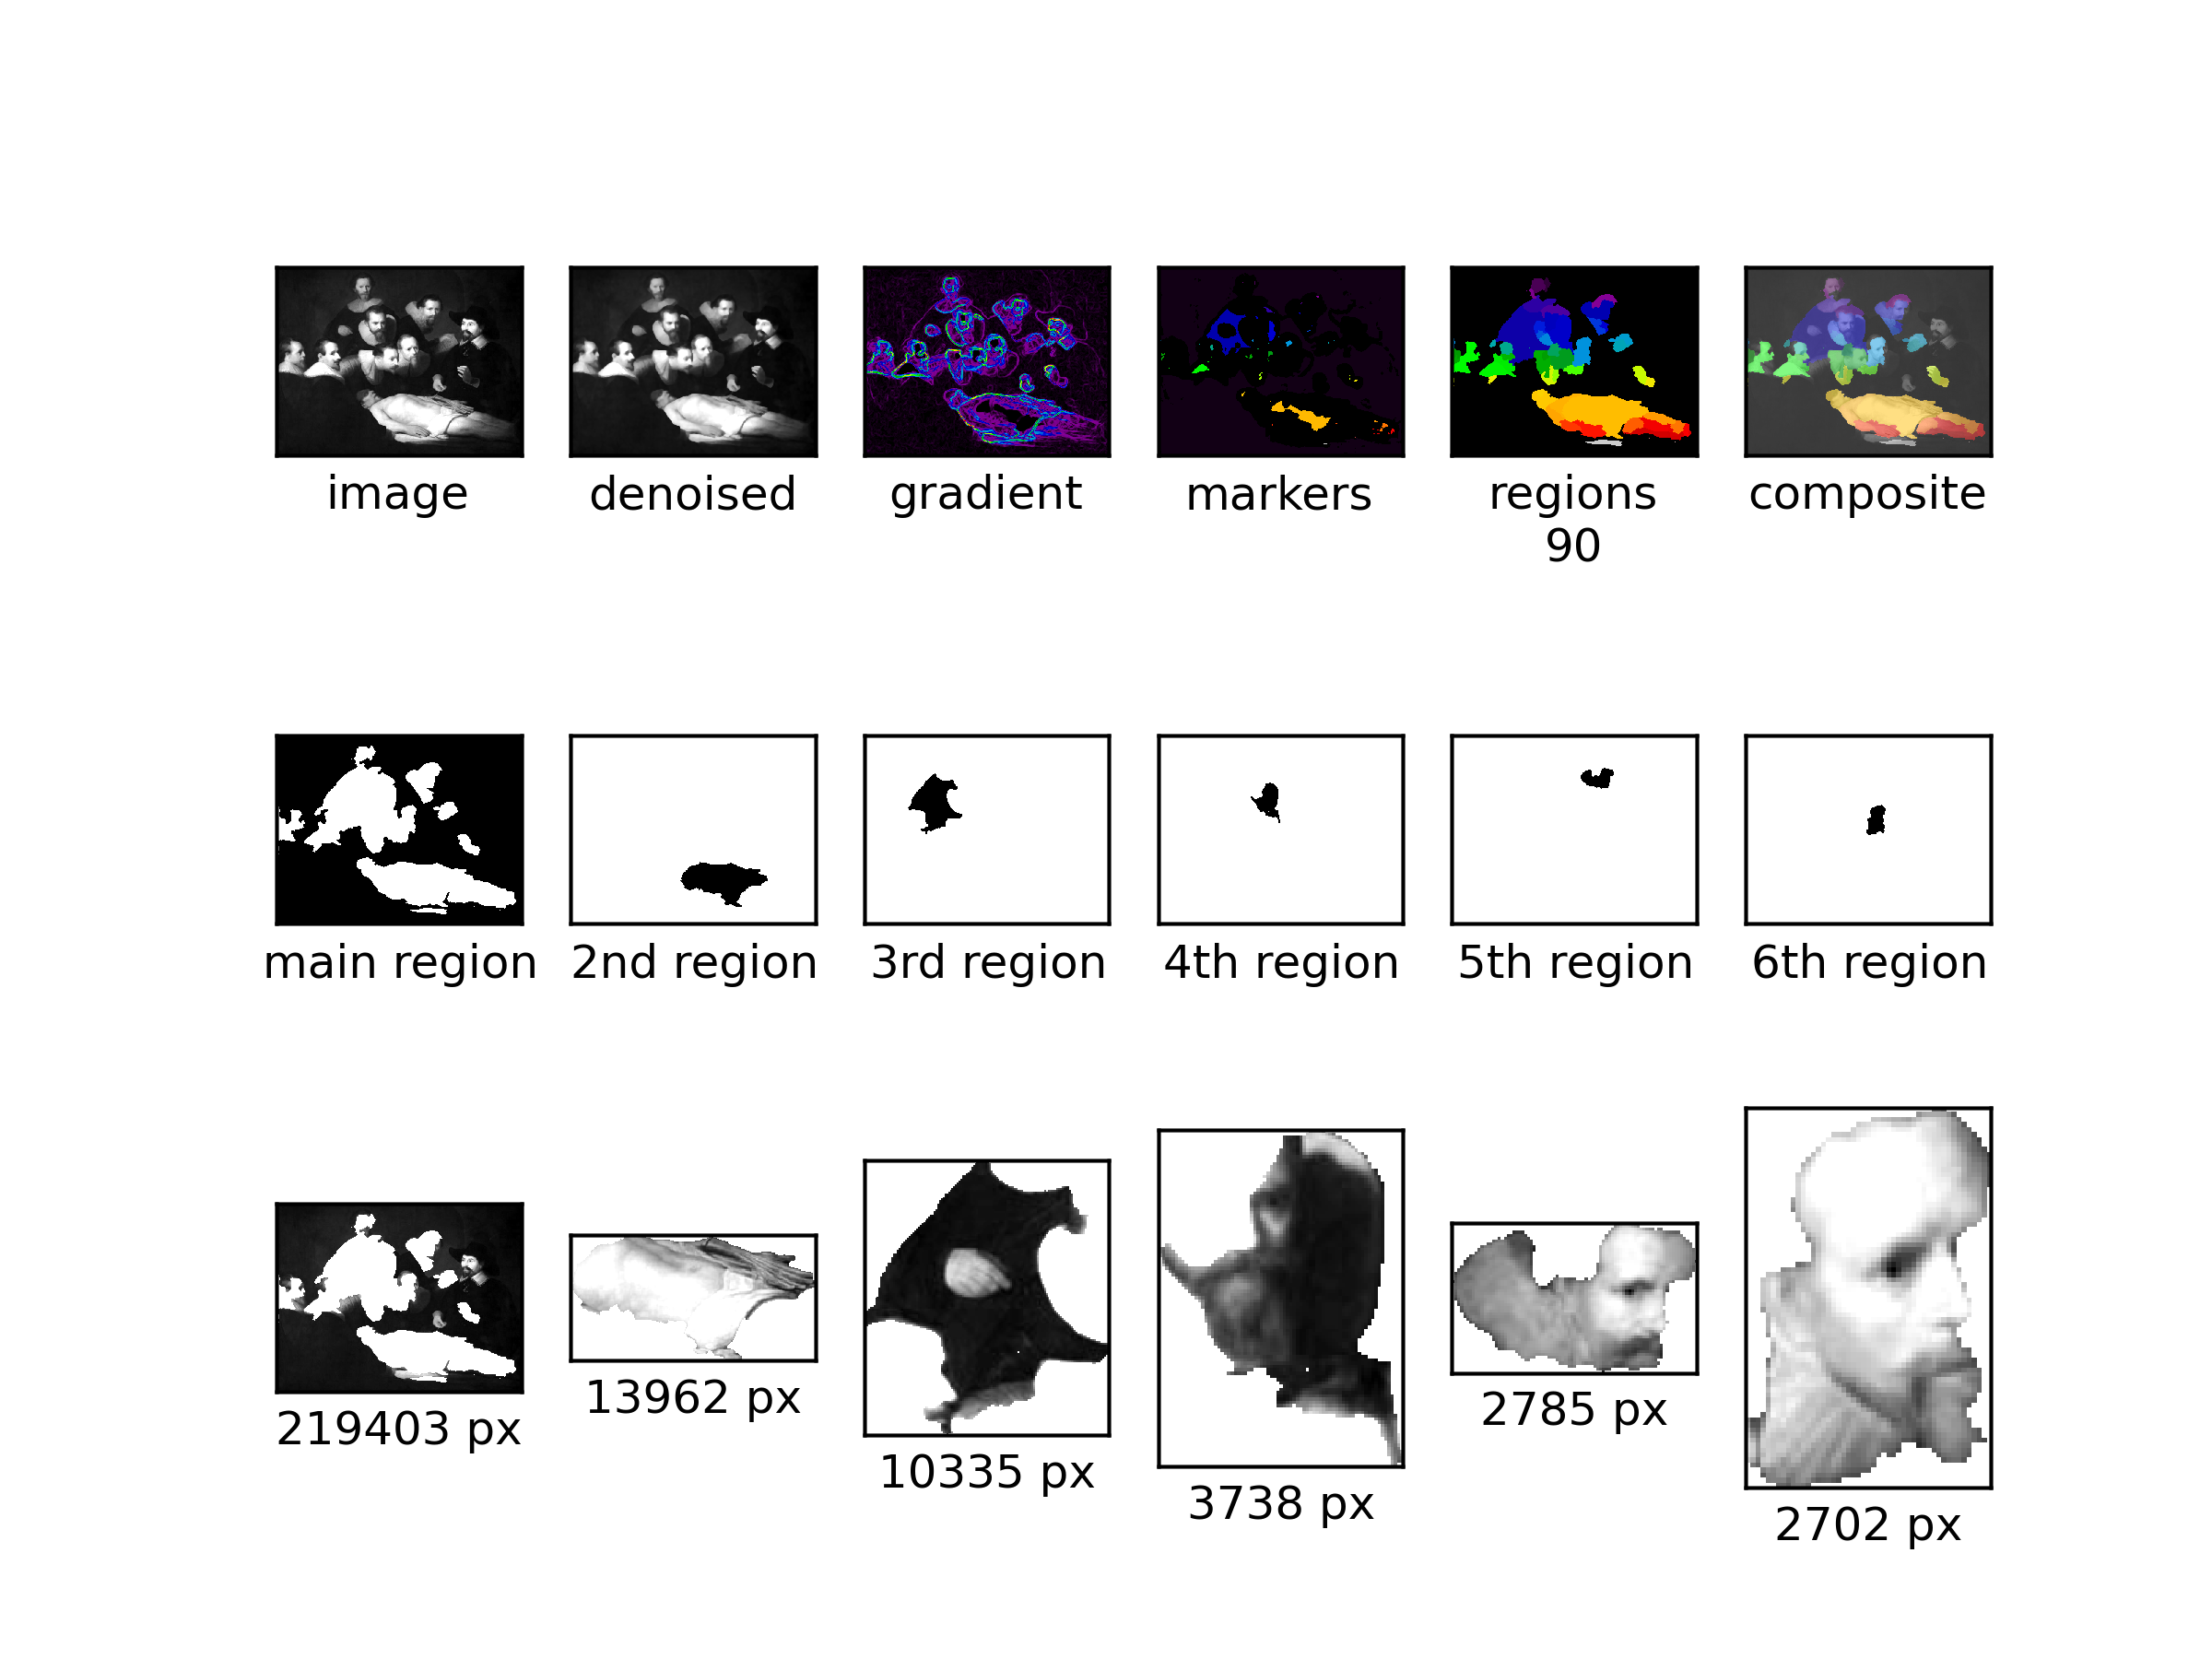
\includegraphics[width=0.9\textwidth]{segm_rembrandt_eu_464}
\caption[Segmentation example]{Segmentation example}
\label{figsegm}
\end{sidewaysfigure*}

\section{Extra Metadata}

It was needed to classify the artists into art movements, some of this data
caould be found on the museum website yet most of it needed to be evaluated by
hand.  The life period and country where the artist worked were the most
important points to classify him into an art movement.

nanan nanan nanan nanan nanan nanan nanan nanan nanan nanan nanan nanan nanan
nanan nanan nanan nanan nanan nanan nanan nanan nanan nanan nanan nanan nanan
nanan nanan nanan nanan nanan nanan nanan nanan nanan nanan nanan nanan nanan
nanan nanan nanan nanan nanan nanan nanan nanan nanan nanan nanan nanan nanan
nanan nanan nanan nanan nanan nanan nanan nanan nanan nanan nanan nanan nanan
batman

\end{multicols}

\chapter{Results and Discussion}

\begin{multicols}{2}

\section{Expected correlation between features}

Artists in the same art movement shall be close, in distinct movements shall be
apart.

nanan nanan nanan nanan nanan nanan nanan nanan nanan nanan nanan nanan nanan
nanan nanan nanan nanan nanan nanan nanan nanan nanan nanan nanan nanan nanan
nanan nanan nanan nanan nanan nanan nanan nanan nanan nanan nanan nanan nanan
nanan nanan nanan nanan nanan nanan nanan nanan nanan nanan nanan nanan nanan
nanan nanan nanan nanan nanan nanan nanan nanan nanan nanan nanan nanan nanan
batman

\section{Measured correlation}

How we calculated the correlation.  Most signiicant numbers from each table.  A
plethora of tables.  A grph with three most prominenet features between each
school.

\begin{table*}[htp]  % table* instead of table because of multicols
\centering
\begin{tabular}{|l|l|}
\hline
Art Movement & Artists \\
\hline \hline
Renaissance    &  Bassano, Botticelli, Raphael, Titian, Veronese             \\
Baroque        &  Berchem, Caravaggio, Cuyp, Dujardin, Greco, Hondecoeter,   \\
               &  Miereveld, Molenaer, Monnoyer, Murillo, Poussin, Rebecca,  \\
               &  Rembrandt, Ribera, Ricci, Rosa, Rubens, Teniers,           \\
               &  Vel\'azquez, Wouwerman                                     \\
Neoclassicism  &  Canaletto, Carlevariis, Dughet, Kauffmann, Panini, Zoffany \\
Romanticism    &  Boudin, Daubigny, Delacroix, Diaz, Gainsborough, Goya,     \\
               &  Latour, Leslie, Loutherbourg, Mulready, Rousseau, Watts    \\
Impressionism  &  Gauguin, Monticelli, Pissarro                              \\
\hline
Watercolour    &  Carpenter, Constable, Tagore                               \\
Mughal         &  Basawan, Jagan, Kesav, La'l, Miskin, Tulsi                 \\
N/A            &  Devi                                                       \\
\hline
\end{tabular}
\caption{Artists in art movements}
\label{sketch}
\end{table*}

nanan nanan nanan nanan nanan nanan nanan nanan nanan nanan nanan nanan nanan
nanan nanan nanan nanan nanan nanan nanan nanan nanan nanan nanan nanan nanan
nanan nanan nanan nanan nanan nanan nanan nanan nanan nanan nanan nanan nanan
nanan nanan nanan nanan nanan nanan nanan nanan nanan nanan nanan nanan nanan
nanan nanan nanan nanan nanan nanan nanan nanan nanan nanan nanan nanan nanan
batman

%\section{meeting: discussion on CBIR (Friday, 1st of July)}
%
%Amount of noise (by random sample) in the cleansed datasets.
%
%Start writing about dataset cleansing heuristics, plus some *descriptions* and
%*statistics*.
%
%Get some of the artists (with most paintings) and do some statistics over
%those.
%
%Histograms of features (especially itten colours) by different artists.
%
%R library to explore data: ggplot2 (use it?).
%
%%%%%%%%%%%%
% Features %
%%%%%%%%%%%%

% Kolmogorov complexity (quality at: 60, 40, 20)
%   JPEG compression: OK!
%   Fractal compression: DON'T BOTHER

% Itten colours
%   saturation, light and dark, extension, complement,
%   hue, warm and cold and simultaneous contrast:       OK!
%
%   harmony: OK!

% Texture (GLCM): OK!
% Edges (sobel and canny filters): OK!
% Rule of thirds: OK!

%%%%%%%%%%%%%%
% Evaluation %
%%%%%%%%%%%%%%

% PCA between pairs of authors
% Pearson correlation coefficient between pairs of authors

%%%%%%%%%%%%%%%%%
% Extrapolation %
%%%%%%%%%%%%%%%%%

% art period/school/movement classification


%nofilter-cs60 nofilter-cs40 nofilter-cs20 nofilter-h60 nofilter-h40
%nofilter-h20 nofilter-l60 nofilter-l40 nofilter-l20 nofilter-shsv60
%nofilter-shsv40 nofilter-shsv20 nofilter-shsl60 nofilter-shsl40 nofilter-shsl20
%nofilter-v60 nofilter-v40 nofilter-v20 sobel-cs60 sobel-cs40 sobel-cs20
%sobel-h60 sobel-h40 sobel-h20 sobel-l60 sobel-l40 sobel-l20 sobel-shsv60
%sobel-shsv40 sobel-shsv20 sobel-shsl60 sobel-shsl40 sobel-shsl20 sobel-v60
%sobel-v40 sobel-v20 canny-cs60 canny-cs40 canny-cs20 canny-h60 canny-h40
%canny-h20 canny-l60 canny-l40 canny-l20 canny-shsv60 canny-shsv40 canny-shsv20
%canny-shsl60 canny-shsl40 canny-shsl20 canny-v60 canny-v40 canny-v20

\begin{sidewaystable*}[ptb]
%\begin{table*}[ptb]
\centering
\begin{tabular}{l|ccccccccc|}
\large{\bf Correlation on Hue}
  & \rotatebox{270}{Kolmogorov raw 60}
  & \rotatebox{270}{Kolmogorov raw 40}
  & \rotatebox{270}{Kolmogorov raw 20}
  & \rotatebox{270}{Kolmogorov Sobel 60}
  & \rotatebox{270}{Kolmogorov Sobel 60}
  & \rotatebox{270}{Kolmogorov Sobel 40}
  & \rotatebox{270}{Kolmogorov Canny 20}
  & \rotatebox{270}{Kolmogorov Canny 40}
  & \rotatebox{270}{Kolmogorov Canny 20}
  \\
\hline
Kolmogorov raw 60  &1.01&2.01&3.01&4.01&5.01&6.01&7.01&8.01&9.01\\
Kolmogorov raw 40  &    &2.01&3.01&4.01&5.01&6.01&7.01&8.01&9.01\\
Kolmogorov raw 20  &    &    &3.01&4.01&5.01&6.01&7.01&8.01&9.01\\
Kolmogorov Sobel 60&    &    &    &4.01&5.01&6.01&7.01&8.01&9.01\\
Kolmogorov Sobel 40&    &    &    &    &5.01&6.01&7.01&8.01&9.01\\
Kolmogorov Sobel 20&    &    &    &    &    &6.01&7.01&8.01&9.01\\
Kolmogorov Canny 60&    &    &    &    &    &    &7.01&8.01&9.01\\
Kolmogorov Canny 40&    &    &    &    &    &    &    &8.01&9.01\\
Kolmogorov Canny 20&    &    &    &    &    &    &    &    &9.01\\
\hline
\end{tabular}
\caption{Artists in art movements}
\label{corrstuff}
\end{sidewaystable*}
%\end{table*}

\end{multicols}

\newpage
\phantomsection
\addcontentsline{toc}{chapter}{\bibname}
\bibliographystyle{plain}
\bibliography{capybara}

\appendix

\chapter{Requirements to run the code}

Describe each library installed, there are some.

nanan nanan nanan nanan nanan nanan nanan nanan nanan nanan nanan nanan nanan
nanan nanan nanan nanan nanan nanan nanan nanan nanan nanan nanan nanan nanan
nanan nanan nanan nanan nanan nanan nanan nanan nanan nanan nanan nanan nanan
nanan nanan nanan nanan nanan nanan nanan nanan nanan nanan nanan nanan nanan
nanan nanan nanan nanan nanan nanan nanan nanan nanan nanan nanan nanan nanan
batman

\chapter{How to run the code}

In an LSB system install the libraries described in (above).  Yu can also clone
the git directl with:

git ...

go to src/ and run the steps in order:

\begin{Verbatim}
./step01
./step02
./step03
./step04
...
\end{Verbatim}

\chapter{jsons tools}

\section{jgrep}

Amount of noise (by random sample) in the cleansed datasets.

Start writing about dataset cleansing heuristics, plus some *descriptions* and
*statistics*.

Get some of the artists (with most paintings) and do some statistics over
those.

Histograms of features (especially itten colours) by different artists.

R library to explore data: ggplot2 (use it?).

\section{jcut}

nanan nanan nanan nanan nanan nanan nanan nanan nanan nanan nanan nanan nanan
nanan nanan nanan nanan nanan nanan nanan nanan nanan nanan nanan nanan nanan
nanan nanan nanan nanan nanan nanan nanan nanan nanan nanan nanan nanan nanan
nanan nanan nanan nanan nanan nanan nanan nanan nanan nanan nanan nanan nanan
nanan nanan nanan nanan nanan nanan nanan nanan nanan nanan nanan nanan nanan
nanan nanan nanan nanan nanan nanan nanan nanan nanan nanan nanan nanan nanan
nanan nanan nanan nanan nanan nanan nanan nanan nanan nanan nanan nanan nanan
nanan nanan nanan nanan nanan nanan nanan nanan nanan nanan nanan nanan nanan
nanan nanan nanan nanan nanan nanan nanan nanan nanan nanan nanan nanan nanan
batman

\section{jcat}

nanan nanan nanan nanan nanan nanan nanan nanan nanan nanan nanan nanan nanan
nanan nanan nanan nanan nanan nanan nanan nanan nanan nanan nanan nanan nanan
nanan nanan nanan nanan nanan nanan nanan nanan nanan nanan nanan nanan nanan
nanan nanan nanan nanan nanan nanan nanan nanan nanan nanan nanan nanan nanan
nanan nanan nanan nanan nanan nanan nanan nanan nanan nanan nanan nanan nanan
nanan nanan nanan nanan nanan nanan nanan nanan nanan nanan nanan nanan nanan
nanan nanan nanan nanan nanan nanan nanan nanan nanan nanan nanan nanan nanan
nanan nanan nanan nanan nanan nanan nanan nanan nanan nanan nanan nanan nanan
nanan nanan nanan nanan nanan nanan nanan nanan nanan nanan nanan nanan nanan
batman

\newpage
\null
\thispagestyle{empty}
\newpage

\end{document}

